\newpage
\criteria{Student Support Services}

\subcriteria{ The student intake policy, admission criteria, and admission procedures to the programme are shown to be clearly defined, communicated, published, and up-to-date.}
\noindent
{\bf การรับนักศึกษา}

	หลักสูตรกำหนดแผนการรับนักศึกษาปีละ 30 คน โดยรกำหนดนโยบายการรับนักศึกษา ช่องทางการรับเข้า คุณสมบัติของนักศึกษาที่จะรับเข้าศึกษา รวมถึงวิธีการคัดเลือกนักศึกษา และได้สื่อสารเผยแพร่ไปยังผู้มีส่วนได้ส่วนเสีย ได้แก่ นักเรียนชั้นมัธยมศึกษาปีที่ 6 ผู้ปกครอง และผู้ที่สนใจทั่วไป ผ่านเว็บไซต์ของมหาวิทยาลัยฯ คณะฯ และของสาขาวิชา รวมทั้ง Facebook ของคณะและสาขาวิชาฯ นอกจากนี้มีการออกประชาสัมพันธ์แนะแนวตามโรงเรียนที่เป็นกลุ่มเป้าหมายและโรงเรียนที่มีความร่วมมือทางวิชาการ (MOU)   กรอบการดำเนินงานเกี่ยวกับการรับนักศึกษาเป็นไปตามที่สำนักส่งเสริมวิชาการและงานทะเบียน (สวท.) เป็นผู้กำหนด เช่น ปฏิทินการรับสมัคร ระบบการสมัครทางระบบออนไลน์ การประกาศผล ฯลฯ ทั้งนี้ในแต่ละปีการศึกษากระบวนการรับนักศึกษามีขั้นตอนการดำเนินการดังนี้
	\begin{enumerate}
		\item งานทะเบียนฝ่ายวิชาการแจ้งให้หลักสูตรจัดทำข้อมูลรายละเอียดการรับสมัครนักศึกษาใหม่ เช่น จำนวนรับ คุณสมบัติผู้สมัคร วิธีการสอบคัดเลือก และคำแนะนำเกี่ยวกับหลักสูตร
		\item หลักสูตรจัดเตรียมข้อมูลเกณฑ์การรับ คุณสมบัติของนักศึกษา และแผนการรับนักศึกษา และส่งให้งานทะเบียนของคณะ 
		\item งานทะเบียนของคณะส่งข้อมูลเกณฑ์การรับ/คุณสมบัติของนักศึกษา แผนรับนักศึกษาไปยัง สวท. ของมหาวิทยาลัย เพื่อนำเข้าสู่การประชุมคณะกรรมการการบริหารวิชาการและวิจัย เพื่อพิจารณาอนุมัติและกำหนดไว้ในคู่มือการรับนักศึกษา
	\end{enumerate}
เมื่อได้รับกสนอนุมัติแผนรับแล้วหลักสูตรดำเนินการตามขั้นตอน วัน-เวลา การดำเนินการของมหาวิทยาลัยต่อไป\\

%%%%%%%%%%%%%%%%%%%%%%
\noindent{\bf เกณฑ์และขั้นตอนการรับเข้า}\\[0.5cm]
หลักสูตรกำหนดเกณฑ์การรับเข้าตามรอบการรับสมัครทั้งหมด 5 รอบ ได้แก่
	\begin{enumerate}
		\item โควตา MOU
		\item TCAS 1
		\item TCAS 2
		\item TCAS 3
		\item TCAS 4
	\end{enumerate}
โดยเกณฑ์และคุณสมบัติของนักศึกษาที่จะรับเข้าในแต่ละรอบมีรายละเอียด\underline{ดังเอกสารหลักฐานระเบียบการรับสมัคร}
และแต่ละรอบมีขั้นตอนและกำหนดการสมัครดังรูป
\ref{Pic6.1-01}\\
\begin{figure}[h!]
	\begin{center}
		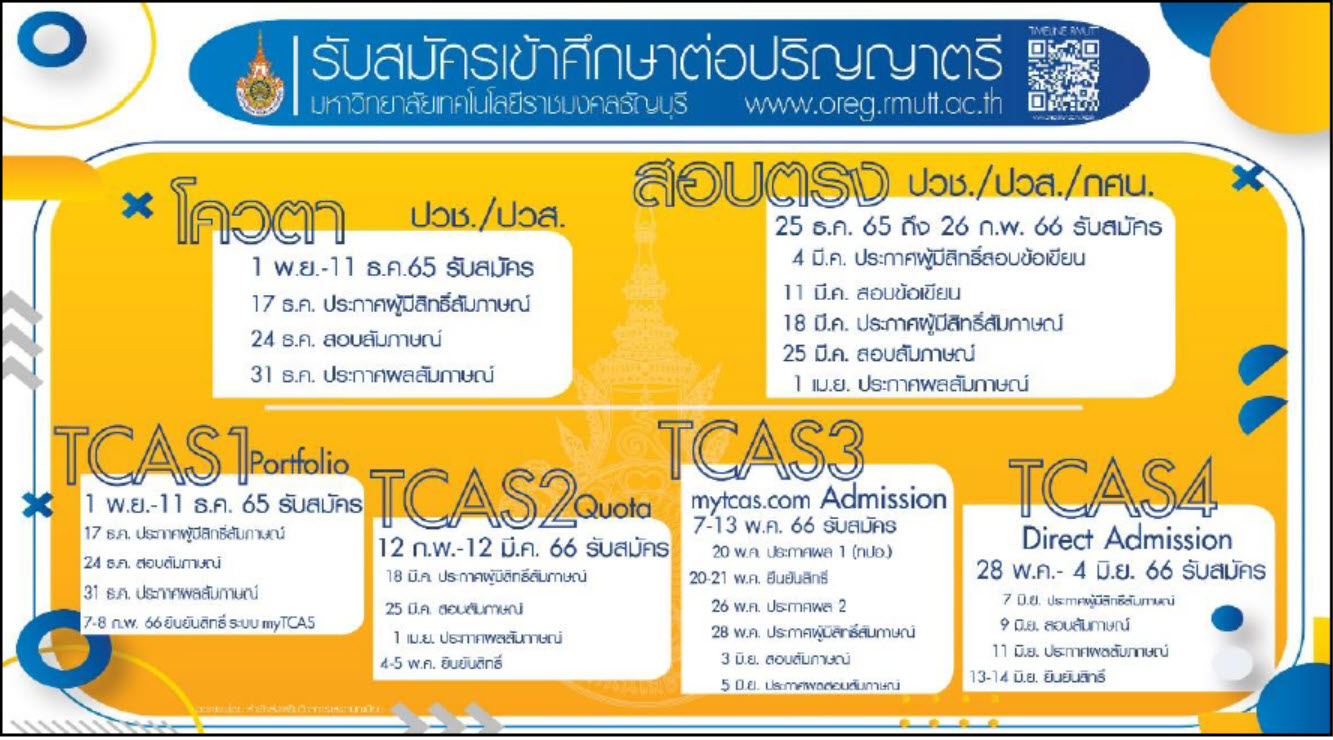
\includegraphics[width=0.9\textwidth]{Pic6.1-01.jpg}
		\end{center}
	\caption{รอบการรับสมัครและช่วงเวลาการรับสมัคร}
	\label{Pic6.1-01}
\end{figure}\\
ผลการดำเนินงานเกี่ยวกับการรับนักศึกษาในปีการศึกษา 2564-2566 หลักสูตรวิทยาศาสตรบัณฑิต สาขาวิชาคณิตศาสตร์ แสดงได้ดังตาราง \ref{table:6.1}
\newpage
\begin{longtable}{ |c|c|c|c|c|c|c|  }
\caption{ข้อมูลเปรียบเทียบแผนรับและจำนวนนักศึกษาที่รายงานตัวปีการศึกษา 2564-2566 }
\label{table:6.1}\\
 \hline
 \multicolumn{7}{|c|}{แผนรับ/รายงานตัว ปีการศึกษา 2564 – 2566} \\
 \hline
  & \multicolumn{2}{c|}{2564} & \multicolumn{2}{c|}{2565} & \multicolumn{2}{c|}{2566} \\
 \hline
 ช่องทางการรับเข้า & แผนรับ & รายงานตัว & แผนรับ & รายงานตัว & แผนรับ & รายงานตัว \\
 \hline
  TCAS 1 & 10 & 6 & 15 & 5 &  15 &   1 \\
 \hline
   TCAS 2& 10 & 3 & 8 & 2 &  7 &   0 \\
 \hline
   TCAS 3& 4 & 5 & 6 & 5 &  7 &  7  \\
 \hline
   TCAS 4 & 2 & 2 & 1 & 2 & 1  & 2   \\
 \hline
 โควตา MOU  & 4 & 18 & - &  9 & -  & 1   \\
 \hline
  รวม  & 30 & 34 & 30 &  23 & 30  &  11  \\
 \hline
\end{longtable}

จากตารางพบว่าแนวโน้มยอดนักศึกษารับเข้าลดลงอย่างต่อเนื่องซึ่งทางหลักสูตรจะดำเนินการปรับปรุงกระบวนการรับเข้าต่อไป
     
  นอกจากนี้หลักสูตรได้สำรวจเกี่ยวกับช่องทางการประชาสัมพันธ์ของนักศึกษาที่รับเข้าในปีการศึกษา 2566 มีผลดังตาราง \ref{table:6.2}
  \newpage
\begin{longtable}{ |>{\raggedright}p{6cm}|c|}
\caption{การรับรู้จากสื่อการประชาสัมพันธ์ของนักศึกษาที่รับเข้าในปีการศึกษา 2566}
\label{table:6.2}\\
 
\hline
\multicolumn{1}{|c|}{{\bf ช่องทางการประชาสัมพันธ์}}     & \multicolumn{1}{c|}{\textbf{ร้อยละของผู้ตอบแบบสอบถาม }}                 \\ \hline
1. เพื่อน  &   11.54\\ 
\hline
2. ครูแนะแนว &   25 \\ 
\hline
3. แนะแนวสัญจร &   11.54 \\ 
\hline
4. เว็บไซค์คณะวิทยาศาสตร์และเทคโนโลยี มทร.ธัญบุรี &  38.46  \\ 
\hline
5. เพจคณะวิทยาศาสตร์และเทคโนโลยี มทร.ธัญบุรี   &   1.92 \\ 
\hline
6. เพจสาขาวิชาคณิตศาสตร์คณะวิทยาศาสตร์และเทคโนโลยี มทร.ธัญบุรี &  5.77  \\ 
\hline
7. อื่นๆ  & 5.77  \\ 
\hline
\end{longtable}

    
 
 \begin{doclist}
 	\docitem{เว็บไซต์/ Facebook การประชาสัมพันธ์}
 	\docitem{ระเบียบการรับสมัครนักศึกษาปีการศึกษา 2566}
 \end{doclist}

%%%%%%%%%%%%%% 6.2 %%%%%%%%%%%%%%%
\subcriteria{Both short-term and long-term planning of academic and non-academic support services are shown to be carried out to ensure sufficiency and quality of support services for teaching, research, and community service.}



หลักสูตรมีการบริการสนับสนุนทางด้านวิชาการและที่ไม่ใช่ทางวิชาการ เพื่อพัฒนาทักษะของนักศึกษาโดยมีการดำเนินการกิจกรรม ตามแผนงานที่จัดทำเพื่อพัฒนาประสบการณ์ ทางวิชาการและวิชาชีพแก่ นักศึกษาโดยมีกิจกรรม ดังนี้\\

\noindent
\textbf{แผนงานระยะสั้น}
\begin{longtable}{ |>{\raggedright}p{3cm}|p{10.5cm}|} 
\hline
\centering{\textbf{กิจกรรม}}   &\multicolumn{1}{c|}{\textbf{รายละเอียด}} \\ \hline
\endhead
1. กิจกรรมบรรยายพิเศษ ในหัวข้อ “Mathematics and statistics in Data Science” โดย Professor Yeol Je Cho   & สาขาวิชาคณิตศาสตร์ร่วมกับสาขาวิชาสถิติประยุกต์ คณะวิทยาศาสตร์และเทคโนโลยี จัดบรรยายพิเศษ ในหัวข้อ “Mathematics and statistics in Data Science” โดย Professor Yeol Je Cho วิทยากรจาก Department of Mathematics Education Gyeongsang National University Jin 52828, KOREA ในวันที่ 26 กรกฎาคม 2566 ณ ห้องประชุมนลินวิทย์ คณะวิทยาศาสตร์และเทคโนโลยี มหาวิทยาลัยเทคโนโลยีราชมงคลธัญบุรีเทคโนโลยี
โดยมีวัตถุประสงค์ ดังนี้ เพื่อให้นักศึกษามีความรู้และความเข้าใจเกี่ยวกับการใช้คณิตศาสตร์และสถิติในการประยุกต์ทางด้าน Data Science
\\ 
\hline
2. กิจกรรมบรรยายพิเศษ ในหัวข้อ "Python for industrial and application" โดยคุณจิรพัฒน์  ลิ้มธนะกุล Western Digital Storage Technologies\newline (Thailand) &   สาขาวิชาคณิตศาสตร์ คณะวิทยาศาสตร์และเทคโนโลยี มหาวิทยาลัยเทคโนโลยีราชมงคลธัญบุรี ได้เปิดสอนรายวิชา 09-114-222 ระเบียบวิธีเชิงตัวเลขเบื้องต้นและรายวิชา 09-114-335 ระบบฐานข้อมูลให้กับนักศึกษาชั้นปีที่ 3 สาขาวิชาคณิตศาสตร์ ในภาคการศึกษาที่ 1/256 โดยในรายวิชา ดังกล่าวมีเนื้อหาเกี่ยวกับการใช้ "Python for industrial and application" จึงได้เชิญคุณจิรพัฒน์  ลิ้มธนะกุล ตำแหน่ง Senior Engineer (Western Digital Storage Technologies (Thailand)) มาเป็นวิทยากรในการบรรยายพิเศษ โดยมีวัตถุประสงค์ ดังนี้ เพื่อให้นักศึกษามีความรู้และความเข้าใจหลักการเบื้องต้นเกี่ยวกับการนำโปรแกรมภาษาไพธอนไปใช้ในอุตสาหกรรม  เพื่อให้นักศึกษามีความรู้และความเข้าใจหลักการเบื้องต้นเกี่ยวกับการนำโปรแกรมภาษา SQL ที่ใช้ในอุตสาหกรรม
   \\ 
\hline
\end{longtable}

\noindent
\textbf{แผนงานระยะยาว}
\begin{longtable}{ |>{\raggedright}p{3cm}|p{10.5cm}|} 
\hline
\centering{\textbf{กิจกรรม}}   & \multicolumn{1}{c|}{\textbf{รายละเอียด}} \\ \hline
1. กิจกรรมเตรียมความพร้อมเข้าสู่รั้วมหาวิทยาลัยและปฐมนิเทศนักศึกษาใหม่ ประจำปีการศึกษา 2566   
& หลักสูตรได้มอบหมายให้อาจารย์ปรึกษาชั้นปีที่ 1 เป็นผู้รับผิดชอบโครงการ โดยมีการให้ความรู้เกี่ยวกับหลักสูตร ระบบงานทะเบียน ตารางเรียน     
เพื่อให้นักศึกษาใหม่ได้ปรับตัวด้านการวางแผนการศึกษาในระดับมหาลัยวิทยาลัย ทั้งด้านวิชาการและการใช้ชีวิต รวมไปถึงให้ความรู้แก่นักศึกษาในเรื่องการเรียนสำหรับรายวิชาที่มีการเขียนโปรแกรม เพื่อให้นักศึกษามีความพร้อมทางด้านการใช้ชีวิตในรั้วมหาวิทยาลัย มีความพร้อมทางด้านการเรียน มีความมุ่งมั่นที่จะเรียน สามารถศึกษาในระดับอุดมศึกษาได้ประสบผลสำเร็จ และสำเร็จการศึกษาได้ตามระยะเวลาที่หลักสูตรกำหนด
\\ 
\hline
2. กิจกรรมสานสัมพันธ์ น้อง-พี่ สาขาวิชาคณิตศาสตร์   
&   หลักสูตรได้จัดกิจกรรมสานสัมพันธ์ น้อง-พี่ สาขาวิชาคณิตศาสตร์ เมื่อวันที่ 15 มกราคม 2567 ซึ่งกิจรรมนี้มีวัตถุประสงค์เพื่อเป็นการกระชับความสัมพันธ์อันดีระหว่างอาจารย์ และนักศึกษา รุ่นพี่-รุ่นน้อง ในสาขาวิชาฯ พร้อมทั้งจัดพิธีมอบทุนการศึกษาให้กับนักศึกษาที่มีผลการเรียนดี และขาดแคลทุนทรัพย์
   \\ 
\hline
3. กิจกรรมแสดงความยินดีกับพี่บัณฑิต  
& หลักสูตรได้จัดกิจกรรมแสดงความยินดีกับพี่บัณฑิต เมื่อวันที่ 13 พฤษจิกายน 2566 โดยมีวัตถุประสงค์เพื่อ แสดงความยินดีกับบัณฑิตของสาขาวิชา ส่งเสริมให้นักศึกษาในสาขาวิชามีความสัมพันธ์ที่ดีต่อกัน ส่งเสริมให้นักศึกษาใหม่ได้รู้จักพี่บัณฑิต อีกทั้งยังเห็นแนวทางในการประกอบอาชีพและเกิดเจตคติที่ดีต่อการเรียนในหลักสูตรฯ
   \\ 
\hline
\end{longtable}


นอกจากนี้ หลักสูตรได้มีการบริการสนับสนุนทางด้านวิชาการและที่ไม่ใช่ทางวิชาการ โดยได้ดำเนินการผ่านฝ่ายพัฒนานักศึกษาโดยมีโครงการ ดังตารางต่อไปนี้

\begin{longtable}{ |>{\raggedright}p{4.5cm}|p{9cm}|} 
\hline
\centering{\textbf{กิจกรรม}}   & \multicolumn{1}{c|}{\textbf{รายละเอียด}} \\
 \hline
 \endhead
1. โครงการ Science game 2023 & ฝ่ายพัฒนานักศึกษา คณะวิทยาศาสตร์และเทคโนโลยี จัดการแข่งขันกีฬา Science Game 2023 ระหว่างวันที่ 8-11 พฤศจิกายน 2566 ณ มหาวิทยาลัยเทคโนโลยีราชมงคลธัญบุรี โดยมีวัตถุประสงค์ดังนี้
\begin{itemize}
 \item เพื่อให้ผู้เข้าร่วมโครงการเห็นคุณค่าของการออกกำลังกายแสดงออกถึงความสามารถด้านกีฬาและทำงานร่วมกันเป็นหมู่คณะ เสริมสร้างคุณธรรมและจริยธรรมยิ่งขึ้น
\item เพื่อเป็นการสร้างสายใยของความรัก ความผูกพัน ความสามัคคี เจตคติที่ดีระหว่างเพื่อน และรุ่นพี่กับรุ่นน้อง เพื่อเกิดการความสัมพันธ์แน่นอนภายในทีมที่สร้างและเสริมสร้างการทำงานร่วมกันอย่างมีประสิทธิภาพ
\item เพื่อสร้างความพร้อมเพรียง สำหรับการซักซ้อมประชุมเชียร์ในการแข่งขันกีฬาต่าง ๆ 
\end{itemize}
\\ 
\hline
2. โครงการเตรียมความพร้อมสู่สถานประกอบการ ภาคการศึกษา 2/2566 & ฝ่ายพัฒนานักศึกษา คณะวิทยาศาสตร์และเทคโนโลยี ได้จัดโครงการเตรียมความพร้อมสู่สถานประกอบการ ภาคการศึกษา 2/2566 วันที่ 16 มีนาคม 2567 โดยมีวัตถุประสงค์คือ เพื่อให้ผู้เข้าร่วมโครงการตระหนักและเห็นความสำคัญของการเตรียมความพร้อมในการสมัครงาน อันเป็นหนึ่งในคุณลักษณะตามบัณฑิตที่พึงประสงค์ KR
   \\ 
\hline
3. โครงการ คิด ลอง ดู เป็นผู้ประกอบการ คณะวิทยาศาสตร์และเทคโนโลยี &  ฝ่ายพัฒนานักศึกษา คณะวิทยาศาสตร์และเทคโนโลยี ได้จัดโครงการ คิด ลอง ดู เป็นผู้ประกอบการ คณะวิทยาศาสตร์และเทคโนโลยี ในวันที่ 14 มีนาคม 2567 เพื่อให้นักศึกษาคณะวิทยาศาสตร์และเทคโนโลยีได้รับการพัฒนาความรู้และทักษะทางด้านแนวคิดการเป็นผู้ประกอบการ
   \\ 
 \hline
4. โครงการปฐมนิเทศนักศึกษาใหม่สานสัมพันธ์พี่น้องคณะวิทยาศาสตร์และเทคโนโลยี ประจำปีการศึกษา 2566 & ฝ่ายพัฒนานักศึกษา คณะวิทยาศาสตร์และเทคโนโลยี ได้จัดโครงการปฐมนิเทศนักศึกษาใหม่สานสัมพันธ์พี่น้องคณะวิทยาศาสตร์และเทคโนโลยี ประจำปีการศึกษา 2566 ระหว่างวันที่ 1-2 กรกฎาคม 2566  โดยมีวัตถุประสงค์
\begin{itemize}
\item เพื่อให้นักศึกษาใหม่มีความเข้าใจบทบาท หน้าที่ และสามารถนำมาใช้เป็นแนวทางการปรับตัวเข้าการเรียนในยุคที่เกิดโรคระบาดโควิด-19 รวมถึงการปรับตัวเข้ากับสังคมระดับอุดมศึกษา
\item เพื่อให้นักศึกษาใหม่ได้รับข้อมูลข่าวสารที่เป็นประโยชน์และสามารถนำไปประยุกต์ใช้ในชีวิตประจำวัน
\item เพื่อให้นักศึกษาใหม่รู้จักสถานที่ภายในรั้วมหาวิทยาลัย คณะ สาขาต่าง ๆ อาจารย์ และเจ้าหน้าที่
\item เพื่อให้นักศึกษาใหม่ได้ทำความรู้จัก และสร้างความสัมพันธ์ รวมถึงการอยู่ร่วมกันด้วยความสามัคคี กับรุ่นพี่ในคณะวิทยาศาสตร์และเทคโนโลยี
\end{itemize} \\
\hline
5. โครงการไหว้ครู คณะวิทยาศาสตร์และเทคโนโลยี ประจำปีการศึกษา 2566 &  ฝ่ายพัฒนานักศึกษา คณะวิทยาศาสตร์และเทคโนโลยี ได้จัดโครงการไหว้ครู คณะวิทยาศาสตร์และเทคโนโลยี ประจำปีการศึกษา 2566 ระหว่างวันที่ 1-2 กรกฎาคม 2566 โดยมีวัตถุประสงค์
\begin{itemize}
\item เพื่อให้นักศึกษาได้แสดงถึงความเคารพนอบน้อมและระลึกถึงพระคุณของครู อาจารย์ 
\item เพื่อสร้างความสัมพันธ์ที่ดีระหว่างครู อาจารย์กับลูกศิษย์
\item นักศึกษาได้เรียนรู้ และรักษาไว้ซึ่งขนบธรรมเนียมประเพณีอันดีงามของไทย
\end{itemize}
   \\ 
\hline
6. โครงการต้นกล้าความดี พัฒนาวิถีชุมชน  & ฝ่ายพัฒนานักศึกษา คณะวิทยาศาสตร์และเทคโนโลยี ได้จัดโครงการต้นกล้าความดี พัฒนาวิถีชุมชน ระหว่างวันที่ 22 มิถุนายน -18 กรกฎาคม 2566 โดยมีวัตถุประสงค์
\begin{itemize}
 \item เพื่อให้ผู้เข้าร่วมโครงการเข้าใจและเห็นคุณค่าของการทำนุบำรุงศิลปวัฒนธรรม 
\item เพื่อให้ผู้เข้าร่วมโครงการได้บูรณาการองค์ความรู้ด้านวิทยาศาสตร์กับการอนุรักษ์ สืบสาน ศิลปวัฒนธรรมภูมิปัญญาท้องถิ่น 
\end{itemize}
 \\ 
\hline
7. โครงการ SciTech Freshy Day & ฝ่ายพัฒนานักศึกษา คณะวิทยาศาสตร์และเทคโนโลยี ได้จัดโครงการต้นกล้าความดี พัฒนาวิถีชุมชน ระหว่างวันที่ 15 มิถุนายน 2566 โดยมีวัตถุประสงค์
\begin{itemize}
	\item เพื่อส่งเสริมให้นักศึกษามีความกล้าแสดงออกและฝึกฝนทักษะทางด้านร่างกาย
\item เพื่อคัดเลือกนักศึกษาที่มีคุณสมบัติเหมาะสมในการเป็นตัวแทนนักศึกษาเพื่อเข้าร่วมการประกวดในระดับมหาวิทยาลัย
\item เพื่อสนับสนุนการใช้เทคโนโลยีให้มีส่วนร่วมในการประชาสัมพันธ์คณะวิทยาศาสตร์และเทคโนโลยีและมีการใช้สื่อไปในทางสร้างสรรค์
\end{itemize}
   \\ 
\hline
\end{longtable}



\begin{doclist}
%	\docitem{เว็บไซต์ www.oreg.rmutt.ac.th}
	\docitem{ภาพ/รายงานการดำเนินกิจกรรม/โครงการของสาขาวิชา}
	\docitem{ภาพ/รายงานการดำเนินกิจกรรม/โครงการของฝ่ายพัฒนานักศึกษา}
\end{doclist}

%%%%%%%%%%% 6.3 %%%%%%%%%%%%%%%%%%%%%%
\subcriteria{An adequate system is shown to exist for student progress, academic performance, and workload monitoring. Student progress, academic performance, and workload are shown to be systematically recorded and monitored. Feedback to students and corrective actions are made where necessary.}


หลักสูตรฯ มีระบบติดตามความก้าวหน้าของนักศึกษา ตรวจสอบผลการศึกษา และภาระการเรียนของนักศึกษา ดังนี้
 \begin{enumerate}
 	\item  หลักสูตรมีระบบการติดตามความก้าวหน้าทางด้านผลการเรียน รายวิชาที่ยังเรียนไม่ครบในหลักสูตร การทดลองคำนวณเกรด โดยนักศึกษาสามารถตรวจสอบข้อมูลได้จากระบบงานทะเบียนของสำนักส่งเสริมวิชาการและงานทะเบียน (www.oreg.rmutt.ac.th) 
 	\item หลักสูตรมีระบบอาจารยที่ปรึกษา โดยแต่งตั้งอาจารย์ที่ปรึกษารายชั้นปี เพื่อวางแผนเกี่ยวกับการดูแลการให้คำปรึกษา โดย
 \begin{enumerate}[label=(\arabic*),leftmargin=0.8cm, labelsep=2mm]
 	\item ก่อนเปิดภาคการศึกษาอาจารย์ที่ปรึกษาให้คำแนะนำเกี่ยวกับการลงทะเบียนเรียน
	\item สัปดาห์แรกของภาคการศึกษา อาจารย์ที่ปรึกษานัดพบนักศึกษาเพื่อพูดคุยและกำหนดวัน-เวลาในการให้คำปรึกษา (Homeroom) 
	\item อาจารย์ที่ปรึกษามีการให้ข้อมูลย้อนกลับแก่นักศึกษาในกรณีที่นักศึกษามีปัญหาทางด้านผลการเรียน และให้คำแนะนำปรึกษาเป็นรายบุคคล โดย
	\begin{itemize}
		\item กรณีที่นักศึกษามีผลการเรียนเฉลี่ยสะสม (GPAX) ไม่ถึง 2.00 จะมีการล็อคระบบการลงทะเบียนของนักศึกษาเพื่อให้นักศึกษามาพบเพื่อให้คำแนะนำและร่วมวางแผนการลงทะเบียนเรียนในแต่ละภาคการศึกษา  
		\item ให้นักศึกษาเข้าพบอาจารย์ที่ปรึกษาเดือนละ 2 ครั้ง เพื่อให้อาจารย์ที่ปรึกษาสามารถติดตามความก้าวหน้าทางการเรียน ให้คำแนะนำและแก้ปัญหาได้ทันเวลา
		\item ให้นักศึกษารายงานผลคะแนนสอบกลางภาคให้อาจารย์ที่ปรึกษาทราบ กรณีที่มีรายวิชาที่นักศึกษาได้คะแนนสอบกลางภาคน้อย อาจารย์ที่ปรึกษาจะแนะนำให้นักศึกษาถอนรายวิชาดังกล่าว 
	\end{itemize}
\item อาจารย์ที่ปรึกษากำกับติดตามและประเมินความเสี่ยงที่อาจเกิดขึ้นในด้านต่าง ๆ นอกเหนือจากด้านผลการเรียนและให้คำแนะนำปรึกษา
\item เมื่อสิ้นสุดภาคการศึกษา ให้อาจารย์ที่ปรึกษาทำสรุปผลการดำเนินงานเสนอต่ออาจารย์ผู้รับผิดชอบหลักสูตร
\item เมื่อสิ้นสุดปีการศึกษา หลักสูตรให้นักศึกษาทุกชั้นปีประเมินความพึงพอใจต่อระบบอาจารย์ที่ปรึกษาซึ่งมี ผลการประเมินแสดงดังตาราง 
\begin{center}
	\begin{tabular}{ |l|c|} 
		%\caption{ผลการประเมินความพึงพอใจของนักศึกษาต่อระบบอาจารย์ที่ปรึกษา}
		%\label{Table:T}
		\hline
		\centering{\textbf{ความพึงพอใจที่มีต่อระบบอาจารย์ที่ปรึกษา}} & \textbf{คะแนนเฉลี่ยความพึงพอใจ} \\
		\hline
		1. ด้านการให้คำปรึกษาเชิงวิชาการ & 4.63  \\ 
		\hline
		2. ด้านการให้คำปรึกษาหรือแจ้งกิจกรรมด้านพัฒนานักศึกษา & 4.62  \\ 
		\hline
		3. ด้านรูปแบบ/เวลาการให้คำปรึกษา & 4.60  \\ 
		\hline
		\textbf{ความพึงพอใจในภาพรวม} & \textbf{4.617}  \\ 
		\hline
	\end{tabular}\\
\end{center}
จากตาราง พบว่า นักศึกษามีความพึงพอใจในภาพรวมอยู่ในระดับพึงพอใจมากที่สุด (คะแนนเฉลี่ย 4.617 จากคะแนนเต็ม 5)\\ 
\item หลักสูตรรวบรวมและสรุปผลการประเมินความพึงพอใจของนักศึกษาและนำผลการประเมินที่ได้ไปปรับปรุงแก้ไขในส่วนที่เกี่ยวข้อง
\end{enumerate}

%\item ระบบกิจกรรมนักศึกษา: มหาวิทยาลัยมีระบบบันทึกชั่วโมงกิจกรรมที่นักศึกษาได้ทำไปแล้ว ซึ่งสามารถตรวจสอบได้ตามจำนวนชั่วโมงที่มหาวิทยาลัยกาหนดจากเว็บไซต์ https://activity.rmutt.ac.th/login.php ในส่วนของอาจารย์ที่ปรึกษาจะคอยช่วยกำกับดูแลนักศึกษาเป็นรายบุคคลเพื่อให้นักศึกษามีชั่วโมงกิจกรรมครบตามที่มหาวิทยาลัยกำหนด
%\begin{figure}[h!]
%    \centering
%    {\includegraphics[width=8.5cm]{6.3-1.png}}
%    \caption{ระบบติดตามชั่วโมงกิจกรรมของนักศึกษา}
%    \label{fig6.3-1}
%\end{figure}
\item หลักสูตรมีการติดตามภาระงาน (workload) ของนักศึกษาเพื่อไม่ให้มีภาระงานมากเกินไป  โดยมอบหมายให้อาจารย์ที่ปรึกษากำกับและติดตามภาระงาน (workload) ของนักศึกษา ซึ่งมีกระบวนการดังนี้
 \begin{enumerate}[label=(\arabic*),leftmargin=0.8cm, labelsep=2mm]
		\item อาจารย์ที่ปรึกษานัดพบนักศึกษา (Homeroom) อย่างน้อยเดือนละ 1 ครั้ง และสอบถามนักศึกษาเรื่องการสั่งงาน/การบ้านของแต่ละวิชา
		\item อาจารย์ที่ปรึกษาพูดคุยกับอาจารย์ผู้สอนแต่ละวิชาเพื่อหาแนวทางในการลดภาระงานของนักศึกษา ยกตัวอย่างเช่น อาจารย์ที่ปรึกษาพูดคุยกับอาจารย์ผู้สอนรายวิชา 09-114-204  การเขียนโปรแกรมคอมพิวเตอร์ทางคณิตศาสตร์ รายวิชา 09-114-223 การสร้างแบบจำลองทางคณิตศาสตร์เบื้องต้น และรายวิชา 09114334 ระบบการจัดเตรียมเอกสารอย่างมืออาชีพ  เพื่อลดภาระงาน (workload) ของนักศึกษา อาจารย์ผู้สอนทั้ง 3 วิชา ได้สั่งงานรายวิชาร่วมกันเป็น 1 ชิ้นงาน  เป็นต้น
	\end{enumerate}

\end{enumerate}






\begin{doclist}
	\docitem{เว็บไซต์ www.oreg.rmutt.ac.th }
	\docitem{แบบบันทึกการเข้ากิจกรรมให้คำปรึกษา (Homeroom)}
\end{doclist}

%%%%%%%%%%% 6.4 %%%%%%%%%%%%%%%%%%%%%%

\subcriteria{Co-curricular activities, student competition, and other student support services are shown to be available to improve learning experience and employability.}

  
\begin{enumerate}
	\item  หลักสูตรได้จัดกิจกรรมเสริมหลักสูตรเพื่อ เพิ่มประสบการณ์ ความรู้และทักษะให้กับนักศึกษา ครอบคลุมทั้งด้านวิชาการและทักษะความสามารถในการทำงาน พร้อมทั้งส่งเสริมการเรียนรู้ตลอดชีวิต โดยมีการกิจกรรมเสริมหลักสูตร ดังนี้\\[3mm]
\begin{tabular}{ |>{\raggedright}p{6cm}|c|c| } 
\hline
\centering{\textbf{ชื่อโครงการ/กิจกรรม}}   & \centering{\textbf{วัน/เดือน/ปี}} &  \textbf{จำนวนผู้เข้าร่วม} \\ \hline
1. กิจกรรมเตรียมความพร้อมเข้าสู่รั้วมหาวิทยาลัยและปฐมนิเทศนักศึกษาใหม่ ประจำปีการศึกษา 2566 &  1 กรกฎาคม 2566 & 59 \\
\hline
2.  กิจกรรมสานสัมพันธ์ น้อง-พี่ สาขาวิชาคณิตศาสตร์ &  15 มกราคม 2567 & 59 \\
\hline
3.  กิจกรรมแสดงความยินดีกับพี่บัณฑิต & 13 พฤษจิกายน 2566 & 72 \\
\hline
\end{tabular}

\item  หลักสูตรส่งเสริมสนับสนุนให้นักศึกษาเข้าร่วมประกวด/แข่งขัน 
โดยในปีการศึกษา 2566 หลักสูตรส่งนักศึกษาเข้าร่วมการประกวดผลงานสหกิจศึกษา-วิทยาศาสตร์ดีเด่น ระดับคณะฯ ประจำภาคการศึกษาที่ 1/2566 จัดขึ้นในวันที่ 7 ธันวาคม 2566 ณ   อาคารเฉลิมพระเกียรติ 6 รอบ พระชนมพรรษา จำนวน 3 ประเภท ดังตารางต่อไปนี้\\[3mm]
  \begin{tabular}{|>{\raggedright}p{3cm}|>{\raggedright}p{5cm}|p{3.5cm}|}
   \hline
   \centering{\textbf{ประเภท}} & \centering{\textbf{ผลงาน}} & \textbf{ชื่อ-นามสกุล นักศึกษา} \\
    \hline
  1. โครงงานสหกิจศึกษา ด้านวิทยาศาสตร์และเทคโนโลยีดีเด่น  & การพัฒนาผลสัมฤทธิ์ทางการเรียนวิชาคณิตศาสตร์ เรื่องเลขยกกำลัง โดยใช้แบบฝึกทักษะ & นางสาวจิรัชญา หัสกัน \\ \hline
   2. โครงงานสหกิจศึกษา ด้านนวัตกรรมดีเด่น  & การพัฒนาสื่อการสอน เรื่อง การคูณพหุนามโดยใช้ CANVA & นางสาวณัฐพร พุทธรักขิโต \\ \hline
   3. โครงงานสหกิจศึกษา ด้านงานประจำดีเด่น & การปฏิบัติงาน ณ แผนก Industrial Engineering (IE) และ แผนก Production (PDT) บริษัท เมย์ยูเม แมนูเฟคเจอริ่ง (ประเทศไทย) จำกัด & นางสาวลดาวัลย์ หารนอก, นางสาวรัตนาภรณ์ รัตนารมภ์ \\ \hline
    \end{tabular}
    
\item หลักสูตรส่งเสริมให้นักศึกษาเข้ารับการทดสอบสมรรถนะจากองค์กรภายนอกในรายวิชา 09114339 วิทยาการข้อมูลสำหรับนักคณิตศาสตร์ อาจารย์ผู้สอนสนับสนุนให้นักศึกษาสอบวัดระดับความสามารถด้านการเรียนรู้เชิงลึกจากองค์กรหรือหน่วยงานที่ได้รับการยอมรับในระดับสากล ผลปรากฏว่านักศึกษาทุกคนที่ลงทะเบียนเรียนวิชานี้ จำนวน 16 คน ได้รับใบประกาศนียบัตรอย่างน้อยหนึ่งใบจาก IBM คิดเป็นร้อยละ 100
\item หลักสูตรส่งนักศึกษาเข้าร่วมกิจกรรมของฝ่ายพัฒนานักศึกษา เพิ่มประสบการณ์ ความรู้และทักษะให้กับนักศึกษา ครอบคลุมทั้งด้านวิชาการและทักษะความสามารถในการทำงาน ดังตารางต่อไปนี้ \\[3mm]
\begin{tabular}{ |>{\raggedright}p{5.8cm}|p{2.2cm}|c|c|} 
\hline
\multicolumn{1}{|c|}{\multirow{3}{*}{\textbf{ชื่อโครงการ/กิจกรรม}}} & \multicolumn{1}{c|}{\multirow{3}{*}{\textbf{วัน/เดือน/ปี}}} &   \textbf{จำนวน}  &   \textbf{ร้อยละความ} \\   
                  &                   & \textbf{ผู้เข้า}  &  \textbf{พึงพอใจในการ}\\   
                  &                   & \textbf{ร่วม}  & \textbf{เข้าร่วมโครงการ}\\ \hline
           
1. โครงการ Science game 2023 & 8-11 พ.ย. 2566 & 400 & 88.5\\
\hline
2.  โครงการเตรียมความพร้อมสู่สถานประกอบการ ภาคการศึกษา 2/2566 & 16 มี.ค. 2567 & 200 & 85\\
\hline
3.  โครงการ คิด ลอง ดู เป็นผู้ประกอบการ คณะวิทยาศาสตร์และเทคโนโลยี & 14 มี.ค. 2567 & 300 & 90.5 \\
\hline
4. โครงการปฐมนิเทศนักศึกษาใหม่สานสัมพันธ์พี่น้องคณะวิทยาศาสตร์และเทคโนโลยี ประจำปีการศึกษา 2566  & 1-2 ก.ค. 2566 & 460 & 84.68\\
\hline
5.  โครงการไหว้ครูคณะวิทยาศาสตร์และเทคโนโลยี ประจำปีการศึกษา 2566 & 16 มีนาคม 2567 & 330 & 90.3\\
\hline
6.  โครงการต้นกล้าความดี พัฒนาวิถีชุมชน & 22 มิ.ย. -18 ก.ค. 2566 &  70 & 90.2 \\
\hline
7.  โครงการ SciTech Freshy Day & 15 มิ.ย. 2566 & 290 & 89.3 \\
\hline
\end{tabular}
\end{enumerate}
\begin{doclist}
	\docitem{ภาพกิจกรรม/รายงานการดำเนินกิจกรรม/โครงการ ของสาขาวิชา }
	\docitem{ใบประกาศนียบัตร }
\end{doclist}


%%%%%%%% 6.5 %%%%%%%%%%%%%%%%%%%%%%%
\subcriteria{The competences of the support staff rendering student services are shown to be identified for recruitment and deployment. These competences are shown to be evaluated to ensure their continued relevance to stakeholders needs. Roles and relationships are shown to be well-defined to ensure smooth delivery of the services.}
\noindent\textbf{การกำหนดสมรรถนะและความสามารถของเจ้าหน้าที่สายสนับสนุน} 

เป็นไปตามกรอบของคณะและมหาวิทยาลัย  โดยคณะมีการจัดทำคำบรรยายลักษณะงาน  (Job Description) คุณสมบัติเฉพาะตำแหน่ง  (Job Specification)  ที่ชัดเจน เกี่ยวกับความสามารถในการให้บริการนักศึกษา มีการกำหนดวิธีการประเมินผลที่มีความ
ชัดเจน เพื่อให้มั่นใจว่า สามารถให้บริการได้อย่างมีประสิทธิภาพแก่ผู้มารับบริการ \\

\noindent\textbf{ระบบการสรรหาบุคลากรสายสนับสนุน}

ในการคัดเลือกบุคลากรสายสนับสนุน คณะฯ ยึดถือตามระเบียบของมหาวิทยาลัยเป็นหลัก และพิจารณาผู้ที่มีคุณสมบัติเฉพาะตำแหน่งเหมาะสมกับงานที่จะได้รับมอบหมาย มีการจัดทำประกาศรับสมัครซึ่งได้กำหนดคุณสมบัติประจำตำแหน่ง บทบาทหน้าที่ ลักษณะงานที่รับผิดชอบ เงินเดือน สวัสดิการ ฯลฯ มีการสื่อสารผ่านทางเว็บไซต์ของคณะและมหาวิทยาลัย\\

\noindent\textbf{การประเมินสมรรถนะของบุคลากรสายสนับสนุน}

ในการประเมินสมรรถนะของบุคลากรสายสนับสนุนจะเป็นการประเมินเพื่อเลื่อนขั้นเงินเดือน  ซึ่งมีการประเมินปีละ 2 ครั้ง (ครั้งที่ 1 คือ 1 ตุลาคม - 31 มีนาคม และ ครั้งที่ 2 คือ 1 เมษายน - 30 กันยายน)  โดยมีคะแนนประเมินจาก 2 ส่วนประกอบคือ 
\begin{enumerate}
\item การประเมินผลสัมฤทธิ์ของบุคลากรสายสนับสนุนในสถาบันอุดมศึกษา มหาวิทยาลัยเทคโนโลยีราชมงคลธัญบุรี คิดเป็นสัดส่วนคะแนน 70\% โดยแบ่งออกเป็น
\begin{itemize}
\item ด้านคุณภาพและปริมาณงาน
\item ด้านความรู้ความสามารถในการปฏิบัติงาน
\item การสร้างผลงานคู่มือปฏิบัติงานหรืองานวิจัย R2R
\item การเข้าร่วมงานและงานมอบหมายอื่น ๆ
\end{itemize}
\item ประเมินสมรรถนะหลักของบุคลากรสายวิชาการที่กำหนดโดยมหาวิทยาลัย 6 ด้าน คิดเป็นสัดส่วนคะแนน 30\% ได้แก่
\begin{enumerate}[label=(\arabic*),leftmargin=0.8cm, labelsep=2mm]
\item รักองค์กรและหน้าที่ มีจิตสำนึก ในการเป็นเจ้าของ เห็นคุณค่าองค์กร มุ่งมั่นการทำงานในหน้าที่อย่างเป็นระบบ มีวินัยและคุณธรรมพัฒนาตนเอง และองค์กรไปสู่เป้าหมายอย่างต่อเนื่อง
\item พัฒนาตนเองเรียนรู้วิทยาการใหม่ๆเพื่อพัฒนาและเพิ่มศักยภาพในการทำงานที่มีประสิทธิภาพและสอดคล้องต่อการเปลี่ยนแปลง มีความรู้ ความเชี่ยวชาญ
\item เป็นมืออาชีพ มีความรู้ ความเชี่ยวชาญ ในการปฏิบัติงาน และเชื่อมโยง แก้ไขปัญหาในการทำงานได้ อย่างเหมาะสมตามจรรยาบรรณวิชาชีพ
\item สื่อสารอย่างสร้างสรรค์ การถ่ายทอดข้อมูลข่าวสารโดยใช้สื่อต่างๆ มีการแลกเปลี่ยนความคิดเห็น และสร้างความเข้าใจร่วมกันในการทำงาน อย่างมีประสิทธิภาพเพื่อพัฒนางาน และองค์กร
\item ทำงานเป็นทีม เปิดใจกว้าง รับฟังความคิดเห็น เรียนรู้และแก้ไข ปัญหาร่วมกันอย่างมีประสิทธิภาพ เพื่อบรรลุเป้าหมายเดียวกัน
\item จิตสาธารณะตระหนักถึงประโยชน์ส่วนรวม ถ่ายทอดความรู้ประสบการณ์ ให้กับองค์กร สังคมชุมชน และประเทศชาติ
\end{enumerate}
\end{enumerate}

โดยมีการกำหนดระดับสมรรถนะที่คาดหวัง ระดับสมรรถนะที่ผู้ถูกประเมินประเมินตนเอง และระดับสมรรถนะที่ประเมินโดยคณะกรรมการประเมิน ซึ่งมีคณะกรรมการ 2 ชุด คือ คณะกรรมการกลั่นกรองขั้นที่ 1 และคณะกรรมการประเมินชุดที่ 2 เป็นผู้ประเมิน
 
ทั้งนี้สาขาวิชาสถิติประยุกต์ร่วมกับสาขาวิชาคณิตศาสตร์มีเจ้าเหน้าที่ธุรการจำนวน 1 คนและเจ้าหน้าที่ดูแลห้องปฏิบัติจำนวน 1 คน ที่รับผิดชอบดูแลงานต่าง ๆ ของทั้ง 2 สาขาวิชาร่วมกัน ในการประเมินการปฏิบัติงานของบุคลากรสายสนับสนุนทั้ง 2 คน จะมีการตั้งกรรมการประเมินเป็นอาจารย์ที่อยู่ในทั้ง 2 สาขาวิชานี้เป็นกรรมการร่วมประเมิน 


นอกจากนี้หลักสูตรยังมีการประเมินความสามารถในการให้บริการผู้เรียนตามสมรรถนะของผู้ให้บริการ ของเจ้าหน้าที่ประจำคณะวิทยาศาสตร์และเทคโนโลยี ซึ่งมีส่วนในการให้บริการด้านการเรียนการสอนและ soft skill ของนักศึกษาได้แก่งานทะเบียนและวัดผล งานกิจกรรมนักศึกษา กีฬาและนันทนาการ งานศิลปวัฒนธรรมและงานวินัยและจริยธรรม
โดยให้นักศึกษาเป็นผู้ประเมิน ซึ่งมีผลการประเมินดังตาราง \ref{Table:T6.5}

   \begin{longtable}{|>{\raggedright}p{9cm}|c|c|c|}
   \caption{ผลการประเมินความสามารถในการให้บริการผู้เรียนตามสมรรถนะของผู้ให้บริการ}	
   \label{Table:T6.5}\\
	\hline
	\centering{\textbf{การให้บริการและช่วยเหลือผู้เรียน}} & \textbf{ค่าเฉลี่ย} & \textbf{S.D.} & \textbf{แปลผล} \\ \hline
	\endfirsthead
	  \caption[]{(ต่อ) ผลการประเมินความสามารถในการให้บริการผู้เรียนตามสมรรถนะของผู้ให้บริการ}	
\\
	\hline
	\centering{\textbf{การให้บริการและช่วยเหลือผู้เรียน}} & \textbf{ค่าเฉลี่ย} & \textbf{S.D.} & \textbf{แปลผล} \\ \hline
	\endhead
	1. \textbf{เจ้าหน้าที่งานทะเบียนและวัดผล} & 4.01 & 0.86 & มาก \\ \hline
	1.1 เจ้าหน้าที่มีความรู้ความสามารถในการตอบปัญหาของผู้รับบริการที่เกี่ยวข้องกับงานทะเบียนและวัดผลได้อย่างถูกต้องชัดเจน & 4.00 & 0.82 & มาก \\ \hline
	1.2 ท่านได้รับคำแนะนำจากเจ้าหน้าที่เกี่ยวกับการยื่นใบคำร้องต่าง ๆ  ได้เป็นอย่างดี เช่น  ใบคำร้องขอเปลี่ยนชื่อ  ขอลาพักการศึกษา  ขอคืนสภาพการเป็นนักศึกษา  การแจ้งสำเร็จการศึกษา  เป็นต้น & 4.03 & 0.86 & มาก \\ \hline
	1.3 เจ้าหน้าที่มีความความรู้ความเข้าใจในระเบียบและข้อบังคับที่เกี่ยวข้องกับงานในความรับผิดชอบ & 3.98 & 0.89 & มาก \\ \hline
	1.4 การติดต่อขอรับบริการของท่านในแต่ละครั้งได้รับการอำนวยความสะดวกจากเจ้าหน้าที่เป็นอย่างดี ไม่มีปัญหา & 4.03 & 0.89 & มาก \\ \hline
	1.5 มีช่องทางให้ติดต่อได้หลายรูปแบบเช่น เว็บไซต์ ระบบขอเอกสารออนไลน์ ไลน์กลุ่ม & 4.00 & 0.91 & มาก \\ \hline
	1.6 เจ้าหน้าที่มีความสามารถในการใช้เทคโนโลยีต่าง ๆ เพื่อการให้บริการ & 4.00 & 0.88 & มาก \\ \hline
	2. \textbf{เจ้าหน้าที่งานกิจกรรมนักศึกษาและงานกีฬาและนันทนาการ} & 3.98 & 0.91 & มาก \\ \hline
	2.1 ความสามารถของเจ้าหน้าที่ในการคำแนะนำนักศึกษาในด้านแหล่งงานนอกเวลา & 3.88 & 0.91 & มาก \\ \hline
	2.2 ความสามารถของเจ้าหน้าที่ในการให้คำแนะนำ/บริการช่วยเหลือนักศึกษาเกี่ยวกับทุนการศึกษา & 3.98 & 0.89 & มาก \\ \hline
	2.3 ความสามารถของเจ้าหน้าที่ในการให้บริการ/คำแนะนำเกี่ยวกับสวัสดิการต่างๆ แก่นักศึกษา & 3.95 & 0.90 & มาก \\ \hline
	2.4 ความสามารถของเจ้าหน้าที่ในการประชาสัมพันธ์และควบคุมดูแลเกี่ยวกับการจัดกิจกรรม/โครงการต่าง ๆ ที่เกี่ยวข้องกับนักศึกษา & 4.03 & 0.92 & มาก \\ \hline
	2.5 เจ้าหน้าที่มีความความรู้ความเข้าใจในระเบียบและข้อบังคับที่เกี่ยวข้องกับงานในความรับผิดชอบ & 4.00 & 0.85 & มาก \\ \hline
	2.6 การติดต่อขอรับบริการของท่านในแต่ละครั้งได้รับการอำนวยความสะดวกเป็นอย่างดี ไม่มีปัญหา & 3.95 & 0.99 & มาก \\ \hline
	2.7 มีช่องทางให้ติดต่อได้หลายรูปแบบเช่น เว็บไซต์ ระบบขอเอกสารออนไลน์ ไลน์กลุ่ม & 4.03 & 0.93 & มาก \\ \hline
	2.8 เจ้าหน้าที่มีความสามารถในการใช้เทคโนโลยีต่าง ๆ เพื่อการให้บริการ & 4.00 & 0.93 & มาก \\ \hline
	3. \textbf{เจ้าหน้าที่งานศิลปวัฒนธรรมและงานวินัยและจริยธรรม} & 4.14 & 0.93 & มาก \\ \hline
	3.1 ความสามารถของเจ้าหน้าที่ในการประชาสัมพันธ์และควบคุมดูแลเกี่ยวกับการจัดกิจกรรมส่งเสริมและสนับสนุนให้นักศึกษามีระเบียบ วินัย ประพฤติปฏิบัติตนตามขนบธรรมเนียมประเพณีและศีลธรรมอันดี & 4.00 & 0.91 & มาก \\ \hline
	3.2 ความสามารถของเจ้าหน้าที่ในการประชาสัมพันธ์และควบคุมดูแลเกี่ยวกับการส่งเสริม และปลูกฝังค่านิยมทางจริยธรรม ค่านิยมทางศาสนา และการปกครองในระบบประชาธิปไตย & 4.03 & 0.95 & มาก \\ \hline
	3.2 ความสามารถของเจ้าหน้าที่ในการประชาสัมพันธ์และควบคุมดูแลเกี่ยวกับการส่งเสริม และปลูกฝังค่านิยมทางจริยธรรม ค่านิยมทางศาสนา และการปกครองในระบบประชาธิปไตย & 4.03 & 0.95 & มาก\\\hline
	3.3 เจ้าหน้าที่มีความความรู้ความเข้าใจในระเบียบและข้อบังคับที่เกี่ยวข้องกับงานในความรับผิดชอบ & 4.10 & 0.98 & มาก\\\hline
	3.4 การติดต่อขอรับบริการของท่านในแต่ละครั้งได้รับการอำนวยความสะดวกเป็นอย่างดี ไม่มีปัญหา & 4.08 & 0.97 & มาก\\\hline
	3.5 มีช่องทางให้ติดต่อได้หลายรูปแบบเช่น เว็บไซต์ ระบบขอเอกสารออนไลน์ ไลน์กลุ่ม & 4.13 & 0.94 & มาก\\\hline
	3.6 เจ้าหน้าที่มีความสามารถในการใช้เทคโนโลยีต่าง ๆ เพื่อการให้บริการ & 4.10 & 0.98 & มาก\\\hline
	3.7 เจ้าหน้าที่มีความความรู้ความเข้าใจในระเบียบและข้อบังคับที่เกี่ยวข้องกับงานในความรับผิดชอบ & 4.10 & 0.96 & มาก\\\hline
	\textbf{เฉลี่ยรวม}&4.02 & 0.91 & มาก\\\hline
\end{longtable}
  จากตารางพบว่านักศึกษามีความพึงพอใจการให้บริการช่วยเหลือผู้เรียนตามสมรรถนะของผู้ให้บริการในภาพรวมอยู่ในระดับมาก (ค่าเฉลี่ยเฉลี่ย 4.02) โดยมีความพึงพอใจน้อยที่สุดในประเด็นความสามารถในการคำแนะนำนักศึกษาในด้านแหล่งงานนอกเวลา  (ค่าเฉลี่ย 3.88 ) ซึ่งทางหลักสูตรจะส่งต่อข้อมูลไปยังคณะเพื่อหาแนวทางปรับปรุงการให้บริการต่อไป 
\begin{doclist}
	\docitem{บรรยายลักษณะงาน  (Job Description) คุณสมบัติเฉพาะตำแหน่ง  (Job Specification) }
	\docitem{การประเมินสมรรถนะของบุคลากรสายสนับสนุน}
	\docitem{ผลการประเมินความคิดเห็นต่อการให้บริการช่วยแหลือผู้เรียนตามสมรรถนะของผู้ให้บริการ}
\end{doclist}
%%%%%%%%%%%%% 6.6 %%%%%%%%%%%%%%%%%%
\subcriteria{Student support services are shown to be subjected to evaluation, benchmarking, and enhancement.}
\noindent
หลักสูตรดำเนินการประเมินความพึงพอใจของนักศึกษาต่อการให้บริการในด้านต่างๆ ได้แก่
\begin{enumerate}
\item การรับนักศึกษาเข้า
\item การพัฒนาศักยภาพนักศึกษาและการส่งเสริมทักษะการเรียนรู้
\item การติดตามความก้าวหน้าและการจัดการเรียนการสอน
\item กิจกรรมเสริมหลักสูตรที่ช่วยเสริมประสบการณ์การเรียนรู้และการได้งาน
\item สมรรถนะของผู้ให้บริการแก่นักศึกษา
\end{enumerate}

เพื่อใช้ในการวางแผนการดำเนินงานและปรับปรุงคุณภาพการให้บริการแก่นักศึกษาโดยมีผลการประเมินดังตาราง \ref{Table:StudentSupSer}
   \begin{longtable}{|>{\raggedright}p{9cm}|c|c|c|}
   	\caption{ผลการประเมินความพึงพอใจของนักศึกษาต่อการให้บริการด้านต่างๆ ปีการศึกษา 2564-2566}
   	\label{Table:StudentSupSer}\\
	\hline
	\multicolumn{1}{|c|}{\textbf{การประเมินความพึงพอใจของนักศึกษา}}&\multicolumn{3}{c|}{\textbf{ปีการศึกษา}}\\
	\cline{2-4}
	&2564&2565&2566\\\hline
	การรับนักศึกษาเข้า&4.52 &4.37 &4.38 \\\hline
	การพัฒนาศักยภาพนักศึกษาและการส่งเสริมทักษะการเรียนรู้ &4.39 &4.30 &4.33 \\\hline
	การติดตามความก้าวหน้าและการจัดการเรียนการสอน&4.48 &4.40 &4.41 \\\hline
	กิจกรรมเสริมหลักสูตรที่ช่วยเสริมประสบการณ์การเรียนรู้\newline และการได้งาน &4.46 &4.39 &4.36 \\\hline
	สมรรถนะของผู้ให้บริการแก่นักศึกษา&- &- & 4.02\\\hline
	
	\end{longtable}

จากตารางพบว่าผลการประเมินความพึงพอใจของนักศึกษาต่อการให้บริการด้านต่าง ๆ มีแนวโน้มลดลงเล็กน้อยในบางประเด็นซึ่งทางหลักสูตรจะนำมาวางแผนปรับปรุงการให้บริการต่อไป
 
สำหรับการเทียบเคียงเพื่อการพัฒนาหรือ Benchmarking กับหน่วยงานอื่นอยู่ในระหว่างการประสานงานเพื่อแลกเปลี่ยนข้อมูล 
\begin{doclist}
	\docitem{ผลการประเมินการความพึงพอใจต่อการให้การบริการ}
	
\end{doclist}









